\chapter{Other low-energy physics with P-type point contact detectors}

In this section, we basically discuss two things: Heavy non-relativistic axions, the signal, and the exclusion limit as calculated with the data from the previous chapter.

Also, making some reasonable assumptions about Majorana, we make some estimates as to the sensitivity of the Majorana experiment to WIMP dark matter and axion dark matter (via the axioelectric effect).  

		
	\section{Other dark matter: heavy axions}
	\label{sec:CalcLimitsOnHeavyAxions}		
		


	\subsection{Heavy axion signal}
	\label{sec:CalcLimitsOnHeavyAxionSignal}		

	The signal for a non-relativistic axion interacting via the axioelectric effect has been derived in~\cite{Pospelov:2008jk}.  This particular inelastic interaction involves the deposition of the \emph{complete} energy of the axion which, in the non-relativistic case, is essentially equal to the mass of the particle.  Since the excitation of the electron via the axioelectric effect is similar to that mediated by a photon in the photoelectric effect, the signal is a delta function centered at the mass of the axion, $m_{a}$.  Convolved with the detector resolution, the signal would appear gaussian with width exactly that of a gamma or x-ray of energy equivalent to $m_{a}$.  The rate of this interaction has been estimated in~\cite{Pospelov:2008jk} as:
	
		\begin{equation}
			R \left[ kg^{-1} day^{-1} \right]\simeq \frac{1.2\times 10^{19}}{A} \gaa^{2} m_a \sigma_{photo}
			\label{eqn:AxioelectricRate}
		\end{equation}

where $A$ is the atomic mass, $m_{a}$ is the mass of the axion in keV, $\sigma_{photo}$ is the measured photoelectric cross section in barns, and $g_{a\bar{e}e}$ is the dimensionless coupling constant.  In the derivation of this result, the value of the density of the dark matter $\rho_{D}$ = 0.3~GeV cm$^{-3}$ was used.  The rate calculated for a germanium detector ($A=72.96$) with a chosen coupling constant, $\gaa = 10^{-11}$, is given in Figure~\ref{fig:HeavyAxionSignalRate}.  The rate calculation used well-known cross sections obtained from the NIST FFAST database located online~\cite{chantler:597}.  

The low noise of PPC detectors yields excellent sensitivity to non-relativistic axions with masses $\leq10$~keV due their sharp resolution at low energies.  A comparison of an axioelectric signal at a given $\gaa$ is provided in Figure~\ref{fig:ResCompare} for characteristic resolutions of NaI and germanium detectors.  In this plot, it is clear that the improved resolution of the germanium detector allows less smearing of the signal, forcing more counts into a narrower peak.

		\begin{figure}
			\centering
			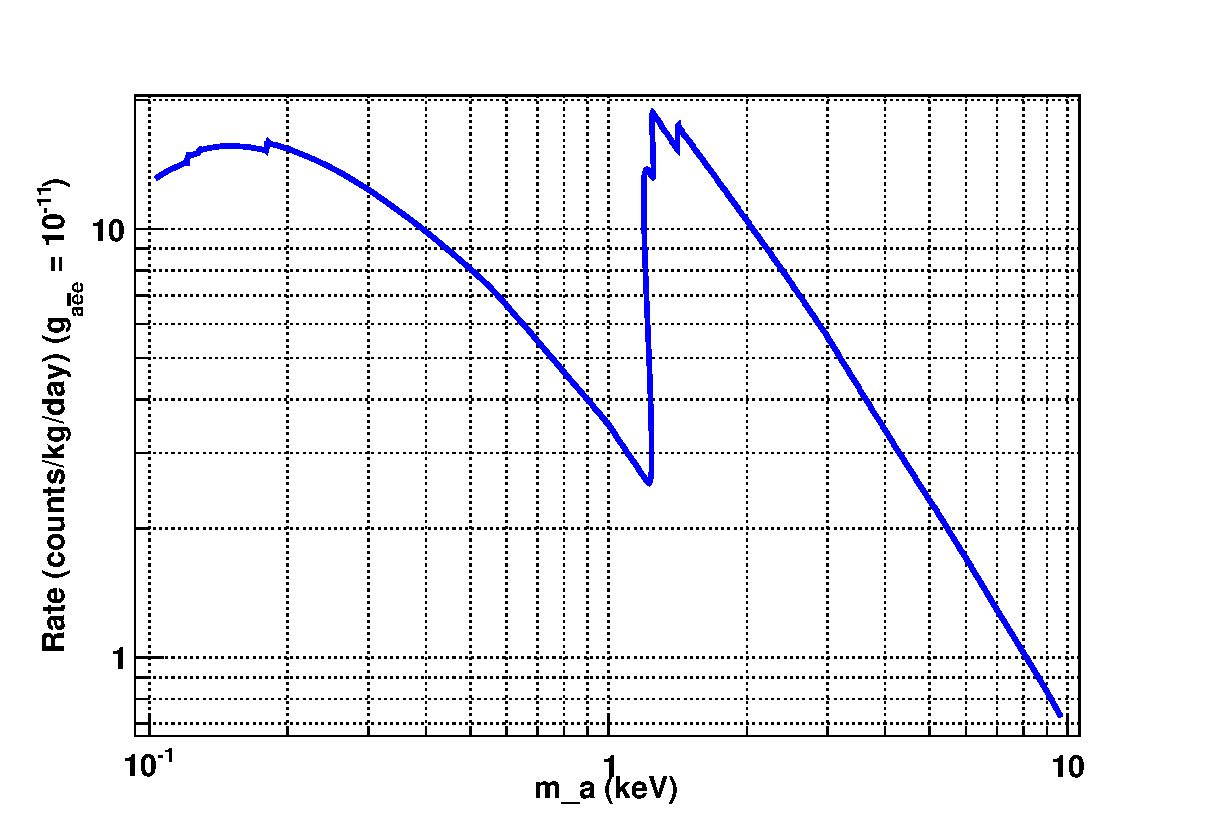
\includegraphics[width=0.9\textwidth]{GeRate}
			\caption[Axioelectric interaction rate in germanium]{Non-relativistic axion axioelectric 
			interaction rate in germanium.  The photoelectric cross section for germanium was obtain
			from the NIST database~\cite{chantler:597}.}
			\label{fig:HeavyAxionSignalRate}
		\end{figure}

		\begin{figure}
			\centering
			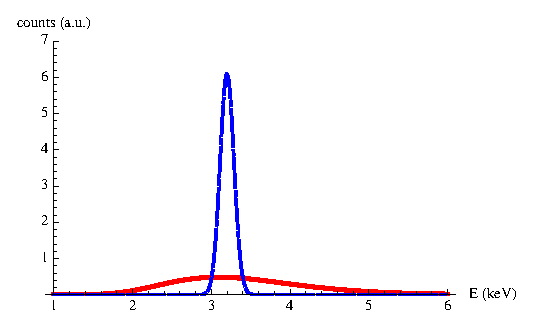
\includegraphics[width=0.9\textwidth]{DAMARes}
			\caption[Axion signal at $m_{a}$ = 3.2~keV]{Axion signal at $m_{a}$ = 3.2~keV comparing 
			the detector responses of germanium (blue, dashed) and NaI (red, solid) to an equivalent
			$\gaa$.  }
			\label{fig:ResCompare}
		\end{figure}

	\subsection{Limits on the axioelectric effect}
	\label{sec:CalcLimitsOnHeavyAxionLimits}		
		
	Limits were calculated using the profile-likelihood method described in Section~\ref{sec:LimitsML}.  Fits were performed on the complete number of data sets described in Chapter~\ref{chap:AnalysisBeGe}, with a total livetime of 150.6~days.  All data sets yielded similar results and so one data set was chosen with 95\% rise-time acceptance cuts and microphonics cuts applied.  As outlined before, assumptions about the source of slow-rise-time events reduced the fidudical mass to 0.33~kg (see Section~\ref{sec:BeGeLowEnergyFeatures}).  Additionally, results with unbinned and binned maximum-likelihood fits were consistent and so the former was used.  The limit calculation followed the same procedure as a peak search in the data and is outlined as follows:
		\begin{itemize}
			\item Define the gaussian signal $f_{axion}$: 
			\begin{itemize}
				\item Choose mass $m_{a}$ of the axion defining $\mu$ of gaussian
				\item Determine $\sigma$ at $E = m_{a}$ using resolution in Equation~\ref{eqn:SigmaEqn}.
			\end{itemize}
			\item Fit to the function $B + N_{axion} f_{axion}$ where $B$ is the background defined in Section~\ref{sec:LimitsDataAndModel} and determine the profile likelihood $\plln$.
			\item Determine the 90\% upper limit on $N_{axion}$ using $\plln$.
			\item Repeat for other values of $m_{a}$
		\end{itemize}		
	
	During the fits, the $\mu$ and $\sigma$ of the gaussian signal, $f_{axion}$, were kept fixed and only the amplitude, $N_{axion}$ was kept as a free parameter of the signal.  For the background, the behavior of the parameters was the same as during WIMP exclusion fits (see Section~\ref{sec:LimitsDataAndModel}) and the relative amplitude of the \gersixeight~and\znsixfive~L-lines was kept fixed as described in Section~\ref{sec:LimitsConstrained}.  Fixing this relative amplitude served to minimize the impact of the L-lines in the exclusion fits since a signal centered at 1.1 and 1.3~keV would look exactly like the L-capture lines.  The difficulties seen while determining limits on low-mass WIMPs did not appear in these calculations because the signal (gaussian centered at $m_{a}$) was not similar to the background except for the case of the L-lines.  The value of the axion mass was scanned from 0.1~keV to 7.8~keV in steps of 0.2~keV using both high- and low-gain channels: high-gain channel, $0.1\to2.9$~keV; low-gain channel, $3\to7.8$~keV.  The axion mass was allowed to vary below threshold (0.5~keV) because the finite resolution of the detector would allow portions of the expected gaussian signal to be detected above threshold.  An example of an exclusion fit in the high-gain channel is shown in Figure~\ref{fig:ExampleHeavyAxionFit} for $m_{a}=3$~keV.  

		\begin{figure}
			\centering
			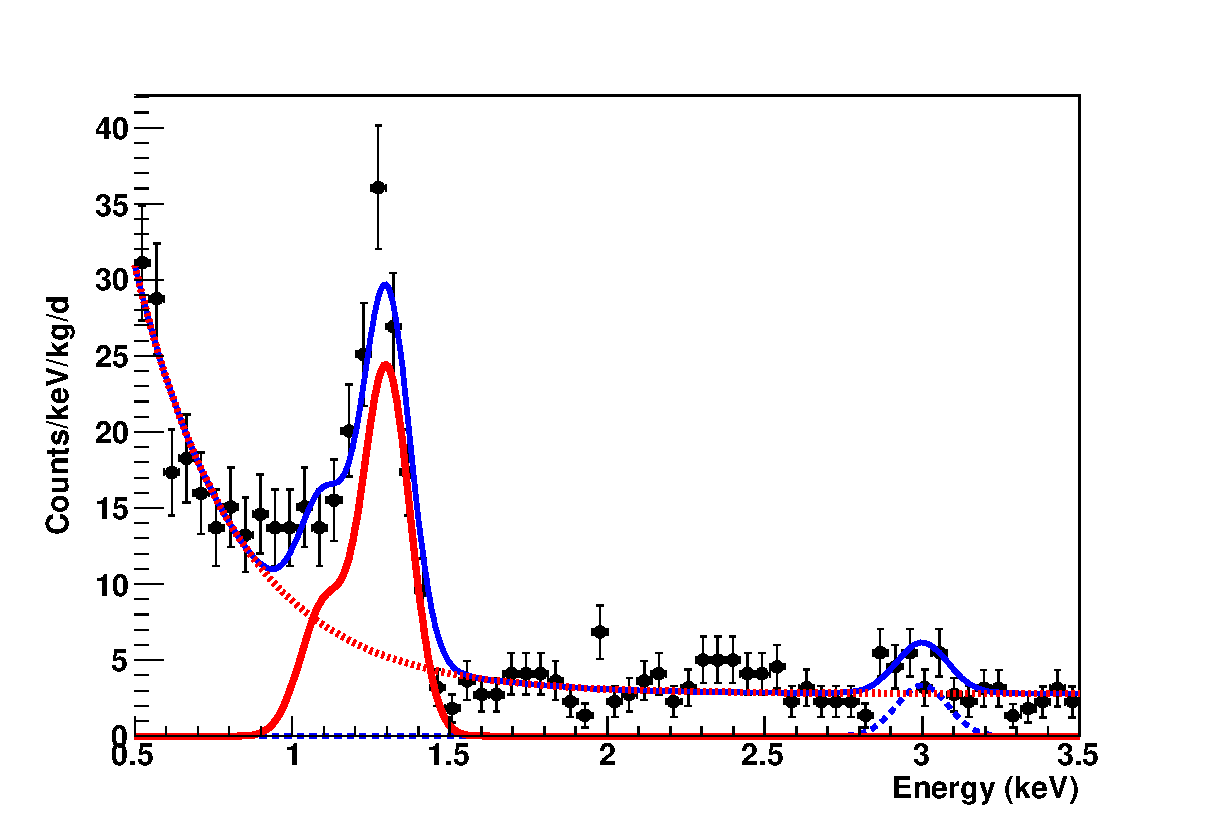
\includegraphics[width=0.9\textwidth]{AxioelectricFitExample}
			\caption[Example of an excluded non-relativistic axioelectric signal at $m_{a}=3$~keV at 
			90\% CL]{Example of an excluded non-relativistic axioelectric signal at $m_{a}=3$~keV at 
			90\% CL.  In this fit performed in the high-gain channel, the excluded value $N_{axion}$ 
			is 36.1 counts.  
			The components of the fits are split: red solid, L-Lines; red dotted, flat plus exponential
			background; blue dashed, excluded axioelectric signal.}
			\label{fig:ExampleHeavyAxionFit}
		\end{figure}
			
	The 90\% CL excluded rate in counts/kg/day, $R_{axion}(m_{a})$, was determined from $N_{axion}(m_{a})$ and from this value the upper limit of $\gaa$ could be determined.  The exclusion calculated from this result is presented in Figure~\ref{fig:HeavyAxionLimits} along with a comparison to other results, including previous results of the CoGeNT collaboration~\cite{Aalseth:2008aa}, the CDMS collaboration~\cite{Ahmed2009}, and an acceptance region from the DAMA collaboration~\cite{Bernabei:2005ca}.  As noted in both references~\cite{Collar:2009sp,Pospelov:2008jk}, the limit calculation performed in~\cite{Bernabei:2005ca} did not correctly treat the leading term in Hamiltonian producing instead a reduced rate for a given $\gaa$ around 3 orders of magnitude lower.  The corrected result from DAMA as outlined in~\cite{Collar:2009sp} appears in Figure~\ref{fig:HeavyAxionLimits}.
			
		\begin{figure}
			\centering
			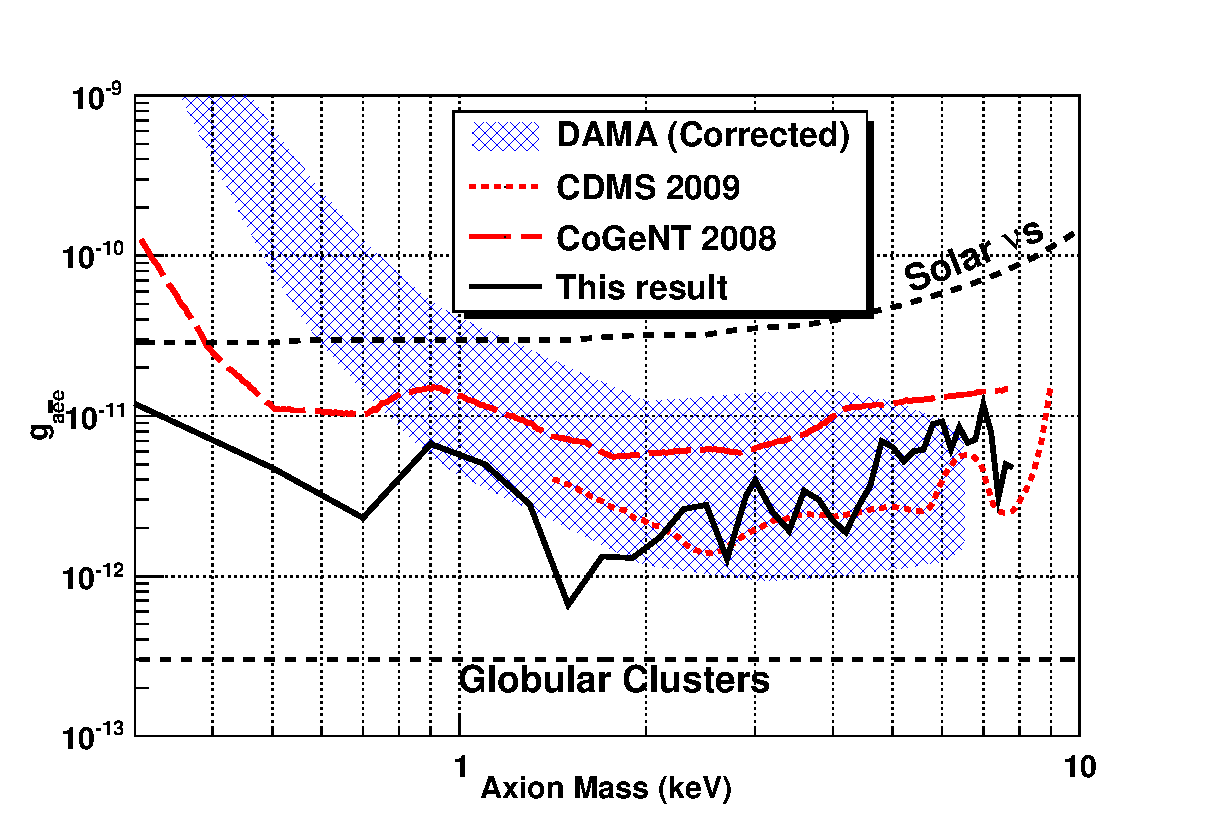
\includegraphics[width=0.9\textwidth]{axion_constrained_unbinnedall_exclusion_plots_final}
			\caption[Limits on the axioelectric coupling constant $\gaa$]{Limits on the axioelectric 
			coupling constant $\gaa$.  Results from this work appear in comparison to previous 
			results from CoGeNT~\cite{Aalseth:2008aa}, CDMS~\cite{Ahmed2009}, and 
			DAMA~\cite{Bernabei:2005ca}.  The DAMA results have been corrected per 
			reference~\cite{Collar:2009sp}.}
			\label{fig:HeavyAxionLimits}
		\end{figure}
		
	\subsection{Conclusions and Discussion}
	\label{sec:DiscOnHeavyAxionLimits}	


							
	\section{Sensitivity of the \MJ~\minmod~to a Dark Matter signal}
	\label{sec:MJSensitivity}
	
	Since a framework was established to determine exclusion limits for low-mass WIMPs and for the axioelectric coupling constant, it is simple to apply this same framework to determine the sensitivities of the \MJ~\minmod.  Calculating the sensitivity of the experiment involves making some assumptions of the background at low energies and of the makeup of the experiment.  A discussion about the estimation of the background is given in the following in Section~\ref{sec:MJLowEnergyBackgroundModel}.  The general prescription for calculating the sensitivity is as follows:
	
		\begin{itemize}
			\item Generate a background model, including an expected rate of background
			\item Simulate a spectrum according to the background model
			\item Fit to the simulated spectrum the background model plus a signal model (e.g.~WIMP or axioelectric spectrum)
			\item Calculate the upper limit on the amplitude of the signal at 90\% CL.
			\item Repeat a large number of times to generate an ensemble of limits.
		\end{itemize}	
From the generated ensemble of limits, the 90\% CL value which was above 99\% of the limits was chosen.  Details of the \MJ~\minmod are given in Chapter~\ref{chap:Majorana}.  For these purposes, we have conservatively assumed that the \MJ~\minmod~will be composed of 20~kg of material and that it will run to accumulate between 1 and 5~years of livetime.  
	
		\subsection{Low-energy background model}
		\label{sec:MJLowEnergyBackgroundModel}
		
The estimation of background generally comes from verified simulations and from extrapolations from previous experiments.  In this work, the background is estimated by assuming it arises from two main sources: (1) a continuum from higher energy processes, and (2) counts from the beta decay of cosmogenically-produced tritium in the detector.  A simulation to estimate (1) is wrought with challenge since a large number of contributions can affect the result.  However, it is possible to use previous results from other germanium-based experiments to produce an estimate of this background.  The IGEX experiment measured a flat background rate of $\sim0.1$~counts/keV/kg/day in this low energy region ($4\to10$~keV)~\cite{Ira01}.    The \MJ~\minmod~plans to reduce background above 200~keV by a factor of 100~\cite{MajoranaWhitePaper} and so it is reasonable to expect the flat background at low energies will follow this same reduction to be roughly 0.001~counts/keV/kg/day.  This background was assumed to not vary in time as well so that it was flat in both time and energy.

The estimate of a background to tritium involves understanding the activation rate of tritium for germanium at the surface of the earth.  This activation rate has been estimated to be $\lesssim200$~\hthree~atoms per kilogram of Ge per day for natural germanium at the surface of the earth, and almost a factor of 2 less for germanium with enriched \gersevensix~content~\cite{Avi92}.  The exposure is determined by the time of manufacture beginning with the pulling of the germanium crystal since the tritium content is `reset' at this point.  For example, if the entire process from crystal pulling to detector development and then final deployment (or storage) underground takes 15~days, then this integrated time is the the total tritium activation period for the detector.  For a kilogram natural-germanium detector created over such a time scale, we would expect there to be $15\times200\sim3000$ atoms of \hthree~within the detector.  Given the slow time of decay of \hthree~(12.32~years), it is critical to minimize the time above ground and certainly necessary to avoid any time at high altitudes, e.g.~storage or transport via airplane.  In this simple background model, two optimistic exposure times are chosen -- 15 and 30~days -- and it is assumed that the detectors begin taking data immediately after arriving underground.  In practice, this assumption is justified due to the long decay time of tritium since the detector will not significantly cool down during a period of time underground much shorter than the lifetime.  The average rates due to these exposures once underground are then roughly 0.03 and 0.06~counts/keV/kg/day for 15 and 30~days, respectively.  The pdf of the tritium decay function was constructed in both time and energy to be:

		\begin{equation}
			f_{^{3}\text{H}}\left(E, t\right)  =  g_{^{3}\text{H}}\left(E\right) \times h_{^{3}\text{H}}\left(t\right) 
		\end{equation}
		with
		\begin{eqnarray}
		g_{^{3}\text{H}}\left(E\right) & = & \sqrt{(E + M_e)^2 - M_e^2} \left(
			E + M_e \right) \left( Q_{^3\text{H}} - E \right)^2 \\
h_{^{3}\text{H}}\left(t\right) & = & e^{-t/\tau_{^3\text{H}}}
		\end{eqnarray}
		and $Q_{^3\text{H}}=18.6$~keV, $M_{e}=511$~keV, and $\tau_{^3\text{H}} = 12.32 / \log(2)$~years.
		
	The background from neutrons has been estimated previously for the IGEX experiment~\cite{Carmona2004523} located at the Canfranc underground laboratory.  This reference considered both neutrons from cosmic-ray muons interacting in the rock as well as neutrons arising from spontaneous fission and ($\alpha$, n) reactions.  Estimates from this (see Figure~7 and Tables 2,3 in\cite{Carmona2004523}, Figure~7 is reproduced here in Figure~\ref{fig:IGEXNeutrons}) suggested that contributions to IGEX from both sources should be below 0.01~counts/keV/kg/day down to 0~keV.  Additionally, it was demonstrated that neutrons from rock radioactivity could be effectively eliminated with additional shielding.  Though the \MJ~\minmod~will have a different geometry to that of the IGEX experiment, it is expected that these numbers are a conservative upper limit due to the fact that the \minmod~will be in a deeper location (DUSEL vs.~Canfranc).  From these conclusions and because the background from \hthree~should at least initially dominate the \minmod, any background contribution from neutrons was omitted from the background model.
	
			\begin{figure}
				\centering
				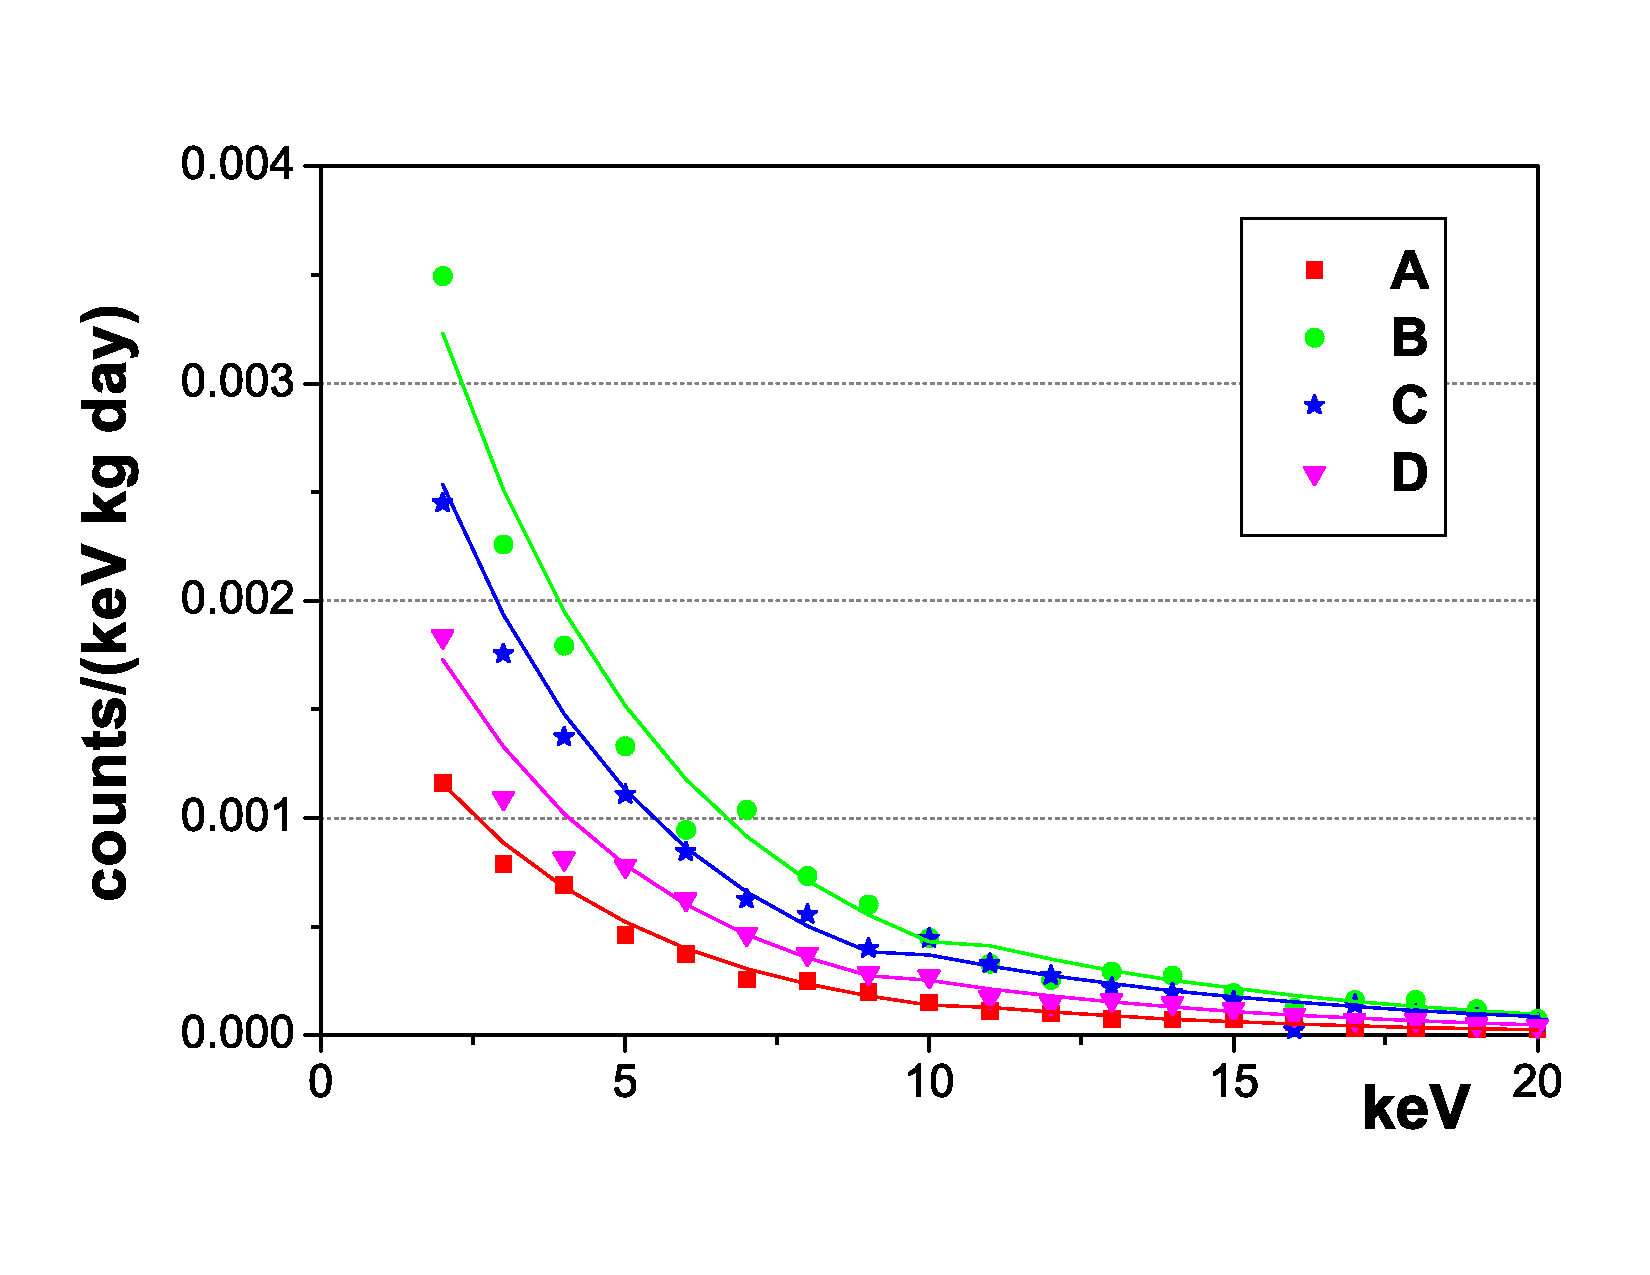
\includegraphics[width=0.9\textwidth]{IGEXNeutronsFromMuons}
				\caption[Simulated muon-induced-neutron spectrum for IGEX.]{Simulated muon-induced-neutron 
				spectrum for IGEX, reproduced from Figure~7 in reference~\cite{Carmona2004523}.  A, B, C, and D are different
				neutron moderator configurations for the IGEX experiment, and the lines are exponential fits to guide the eye.
				A conservative extrapolation suggests that all of these spectra should be well below 0.01~counts/keV/kg/day at
				0~keV and is much less than 0.001~counts/keV/kg/day above 10~keV.}
				\label{fig:IGEXNeutrons}
			\end{figure}
	
	In general, the detector response must be convolved with the spectrum to get a realistic shape.  However, since point-contact detectors have such excellent energy resolution ($\sigma\sim70$~eV, the response has limited effect on the spectra.  Therefore, no correction for finite resolution was taken into account.  

		\subsection{Sensitivity Fitting}
		\label{sec:MJSensitivityFitting}
	
	The fitting procedure used binned maximum likelihood instead of an unbinned fit to reduce the time required in estimating an upper limit for each toy data model.  Three parameters affecting the fits were varied: tritium exposure time, threshold, and exposure time of the \minmod.  Each of these parameters could take two different values (see Table~\ref{tab:SensFitValues}) so that for each signal eight different sets of fits were done.  The data sets and fitting pdfs were both fully two-dimensional in energy and time and were fit over a range from threshold to 20~keV.  The binning was chosen as follows: 64~bins for energy and 16~bins for time.  For each of the eight set of fits for a signal, an ensemble of upper limits with a population $\gtrsim1500$\footnote{ An exact population number was not specified for the ensembles to maximize the efficiency of the calculation.  It was more efficient to specify the \emph{time} for the calculation to run, than for to define a specific number of iterations.} was generated on the Athena cluster at the University of Washington~\cite{Athena}.  The final sensitivity calculations outlined in the following sections took roughly 700 hours of real-time or 221~cpu-days.
	
			\begin{table}
				\centering
				\begin{tabular}{l r}
					\toprule
					Variable & Values \\
					\midrule
					\hthree~exposure time & 15, 30~days \\
					Threshold & 0.3, 0.5~keV \\
					\minmod~exposure & 1, 5~years (20, 100~kg-years) \\
					\bottomrule 
				\end{tabular}				
				\caption[Variations on background and fitting for \MJ~\minmod~sensitivity calculations]
				{Variations on background and fitting for \MJ~\minmod~sensitivity calculations}
				\label{tab:SensFitValues}
			\end{table}		
		
		\subsection{Sensitivity to WIMPs}
		\label{sec:MJSensitivityToWIMP}
		
		Make comments on the shape of the excluded distribution with reference to the different 
		
	The sensitivity calculations employed the 2-dimensional (time, energy) signal described in the previous chapter and more details can be found in Section~\ref{sec:CalcLimitsOnWIMPSignal}.  The equivalent values for all constants in the WIMP signal were used as previously noted.  The fits proceeded as outlined in the previous section (Section~\ref{sec:MJSensitivityFitting}).  The shape of the WIMP signal was parameterized solely by the mass of the WIMP, $M_{W}$, and so fits were performed with different values of this parameter on a variable grid (in GeV): 2.9; 3; 3.5; $4\to10, \Delta M_{W} = 1$; $12\to24, \Delta M_{W} = 2$; $30\to100, \Delta M_{W} = 10$; $100\to1000, \Delta M_{W} = 100$.  An example sensitivity fit to a WIMP signal at $M_{W}=10$~GeV is given in Figure~\ref{fig:MJSensitivityToWIMPExample}.  In this particular example, the threshold was 0.3~keV, \hthree~exposure time was 15~days, and the total exposure time was 1~year.  It is clear that the amplitude of the excluded signal is very small and perhaps smaller than one might expect given the average count rate dominated by the \hthree~decay.  However, the shape of a WIMP signal is significantly different from that of a tritium beta spectrum making a stronger exclusion possible because the shape of the spectra are taken into account.  A simple integration analysis looking solely at counts in a defined energy window would fail to produce the same limits.  
		
			\begin{figure}
				\centering
				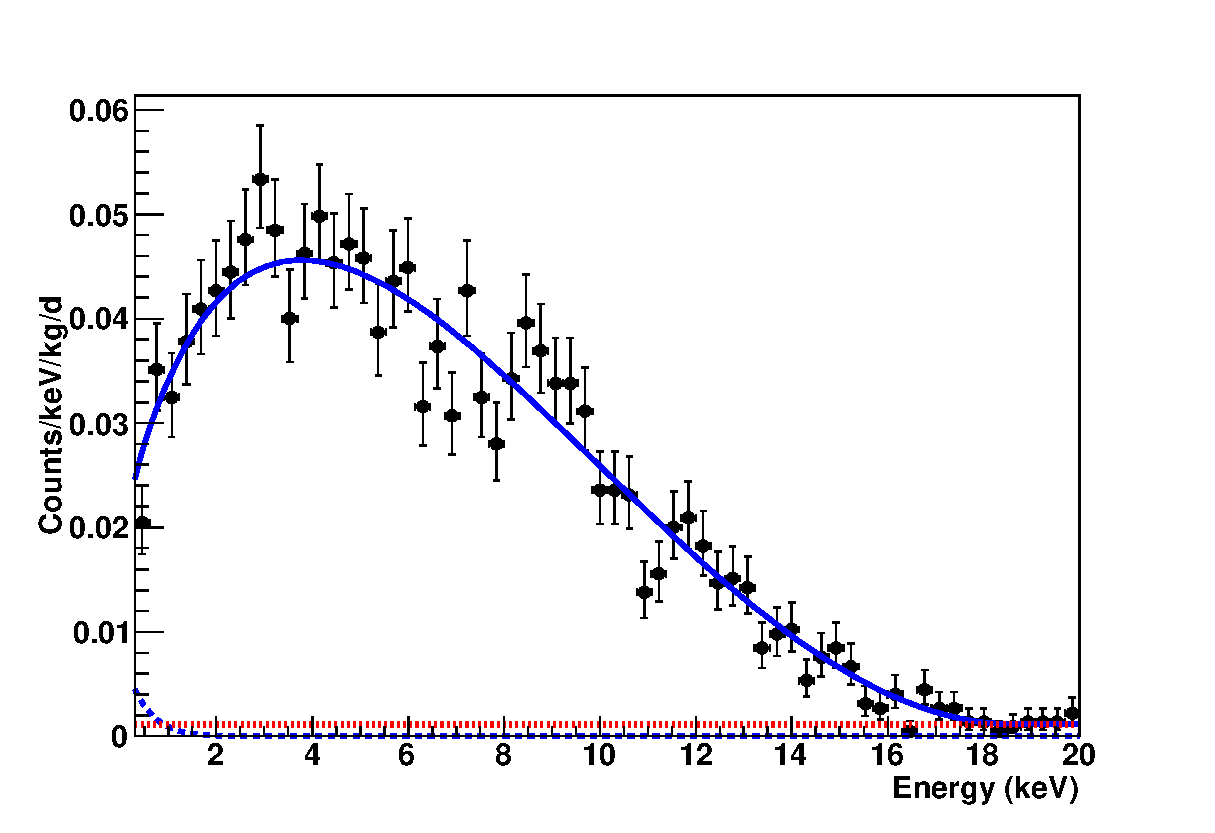
\includegraphics[width=0.9\textwidth]{MJDemoExampleSensFit}
				\caption[\MJ~\minmod WIMP sensitivity fit example.]{A sensitivity fit example with WIMP  
				signal at $M_{W}=10$~GeV, with $\signuc$ excluded at 90\% CL with value
				 $8.6\times10^{-9}$~pb.  Components of the fit are broken out including WIMP 
				 signal (blue dashed) and flat background (red dotted).  The beta spectum from \hthree~dominates the fit.}
				\label{fig:MJSensitivityToWIMPExample}
			\end{figure}
	
	The final results of the sensitivity calculation are presented in Figure~\ref{fig:MJSensitivityToWIMP}.  This figure includes results from the eight different sets of fits with the modification of the exposure times and the threshold.  All the exclusion plots exhibit a similar characteristic shape including a small dip in the $M_{W} = 4 \to 6$~GeV region.  This `dip' is due to the sharp reduction of the tritium spectrum at low energies and because the WIMP signal in this mass range is a very steep exponential.  Counterintuitively, in this region the `dip' for larger tritium exposure times yields a better exclusion limit.  It is expected that this occurs because the larger number of events in the beta spectrum yields a better measurement of its amplitude and reduces the uncertainty in the measurement near threshold.  Aside from this, the factor of 2 increase in exposure time doesn't have a significant impact other than slightly softening the exclusion limits.  In contrast, the threshold has a significant impact below 10.5~GeV yielding much better exclusions for WIMP masses below that value.  This is certainly due to the sharp reduction of the tritium spectrum at low energies and to the sharp turn on of the exponential-like WIMP spectrum.  As expected, the reduced threshold of 0.3~keV enables limits to be made down to $M_{W}=3$~GeV.
	
			\begin{figure}
				\centering
				\def\figheight{0.41\textheight}				
				\subfigure[1~year (20 kg-yr) exposure time]{
					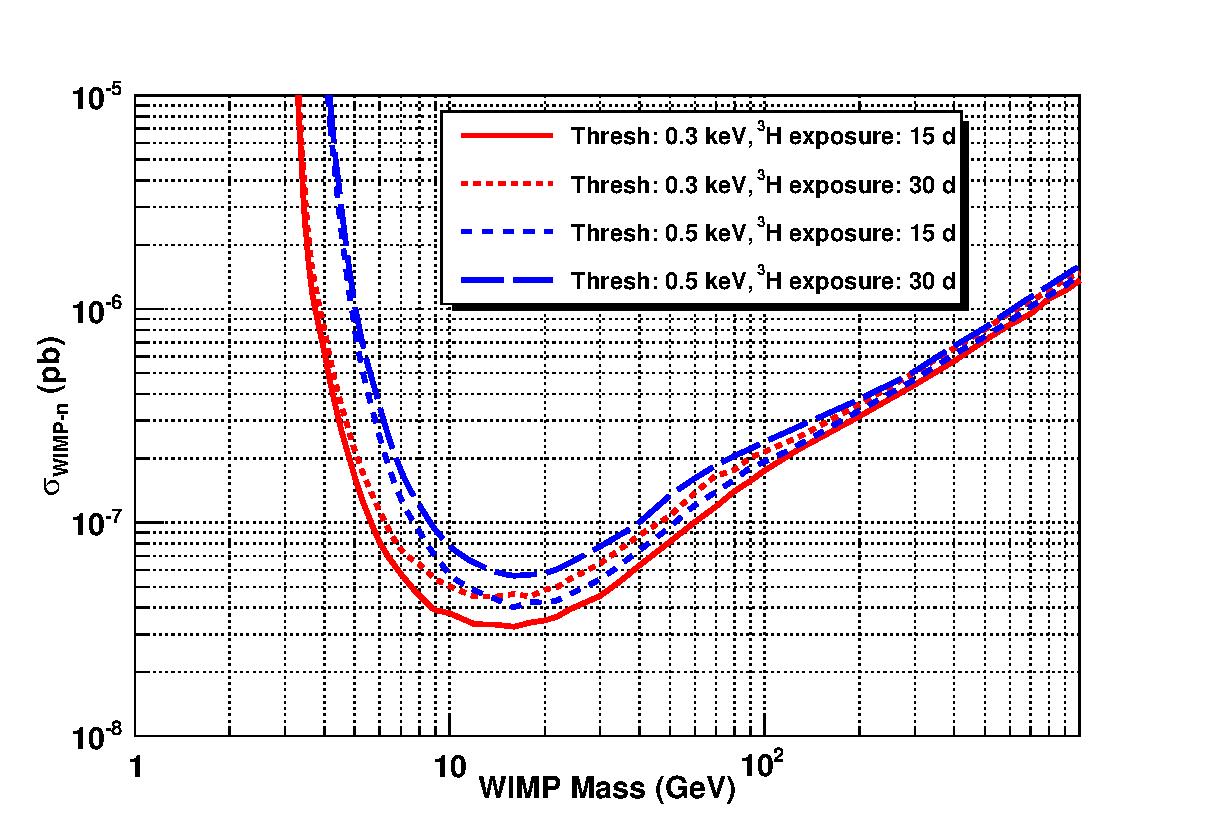
\includegraphics[height=\figheight]{20TimeExposureMJ}
					\label{fig:20TimeExposureMJ}						
				}
				\subfigure[5~year (100 kg-yr) exposure time]{
					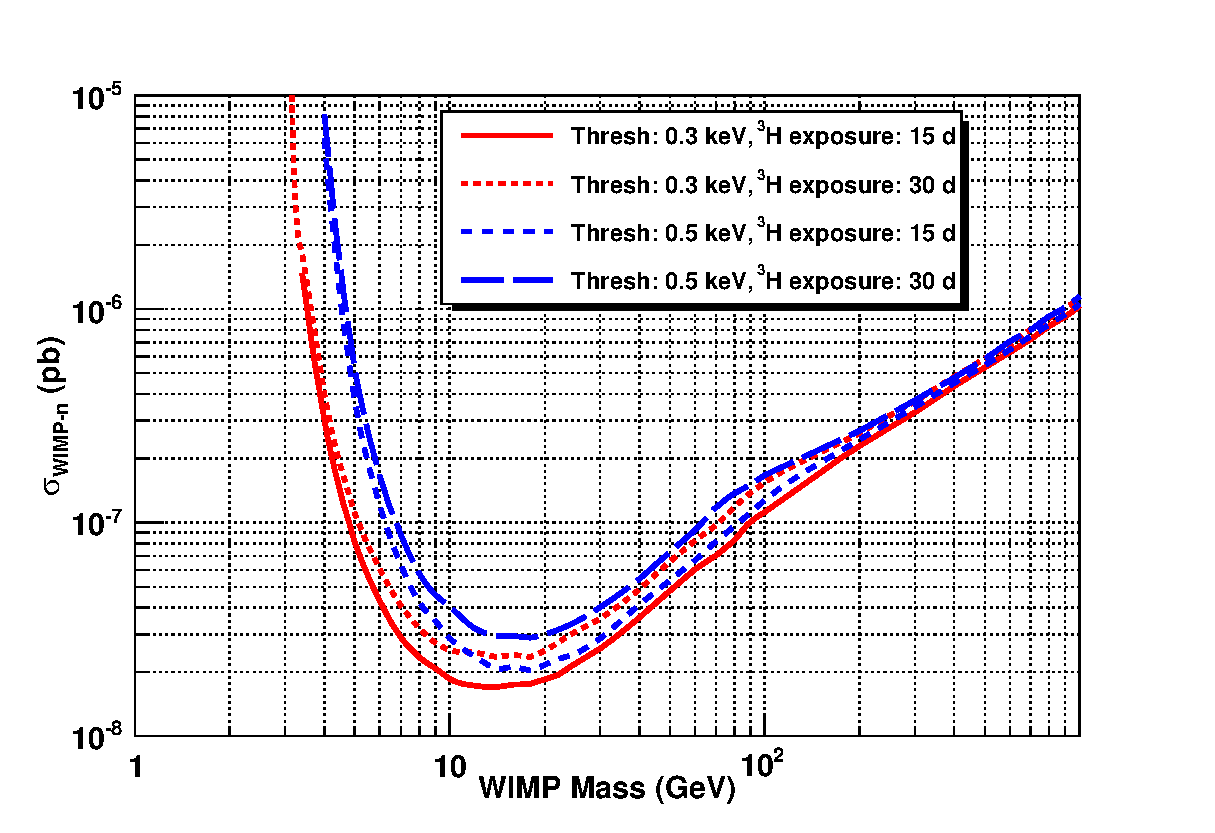
\includegraphics[height=\figheight]{100TimeExposureMJ}
					\label{fig:100TimeExposureMJ}						
				}				
				\caption[\MJ~\minmod~sensitivity to a WIMP signal]{\MJ~\minmod~sensitivity.  Lines are 90\% confidence level exclusions.}
				\label{fig:MJSensitivityToWIMP}
			\end{figure}		
		
			\begin{figure}
				\centering
				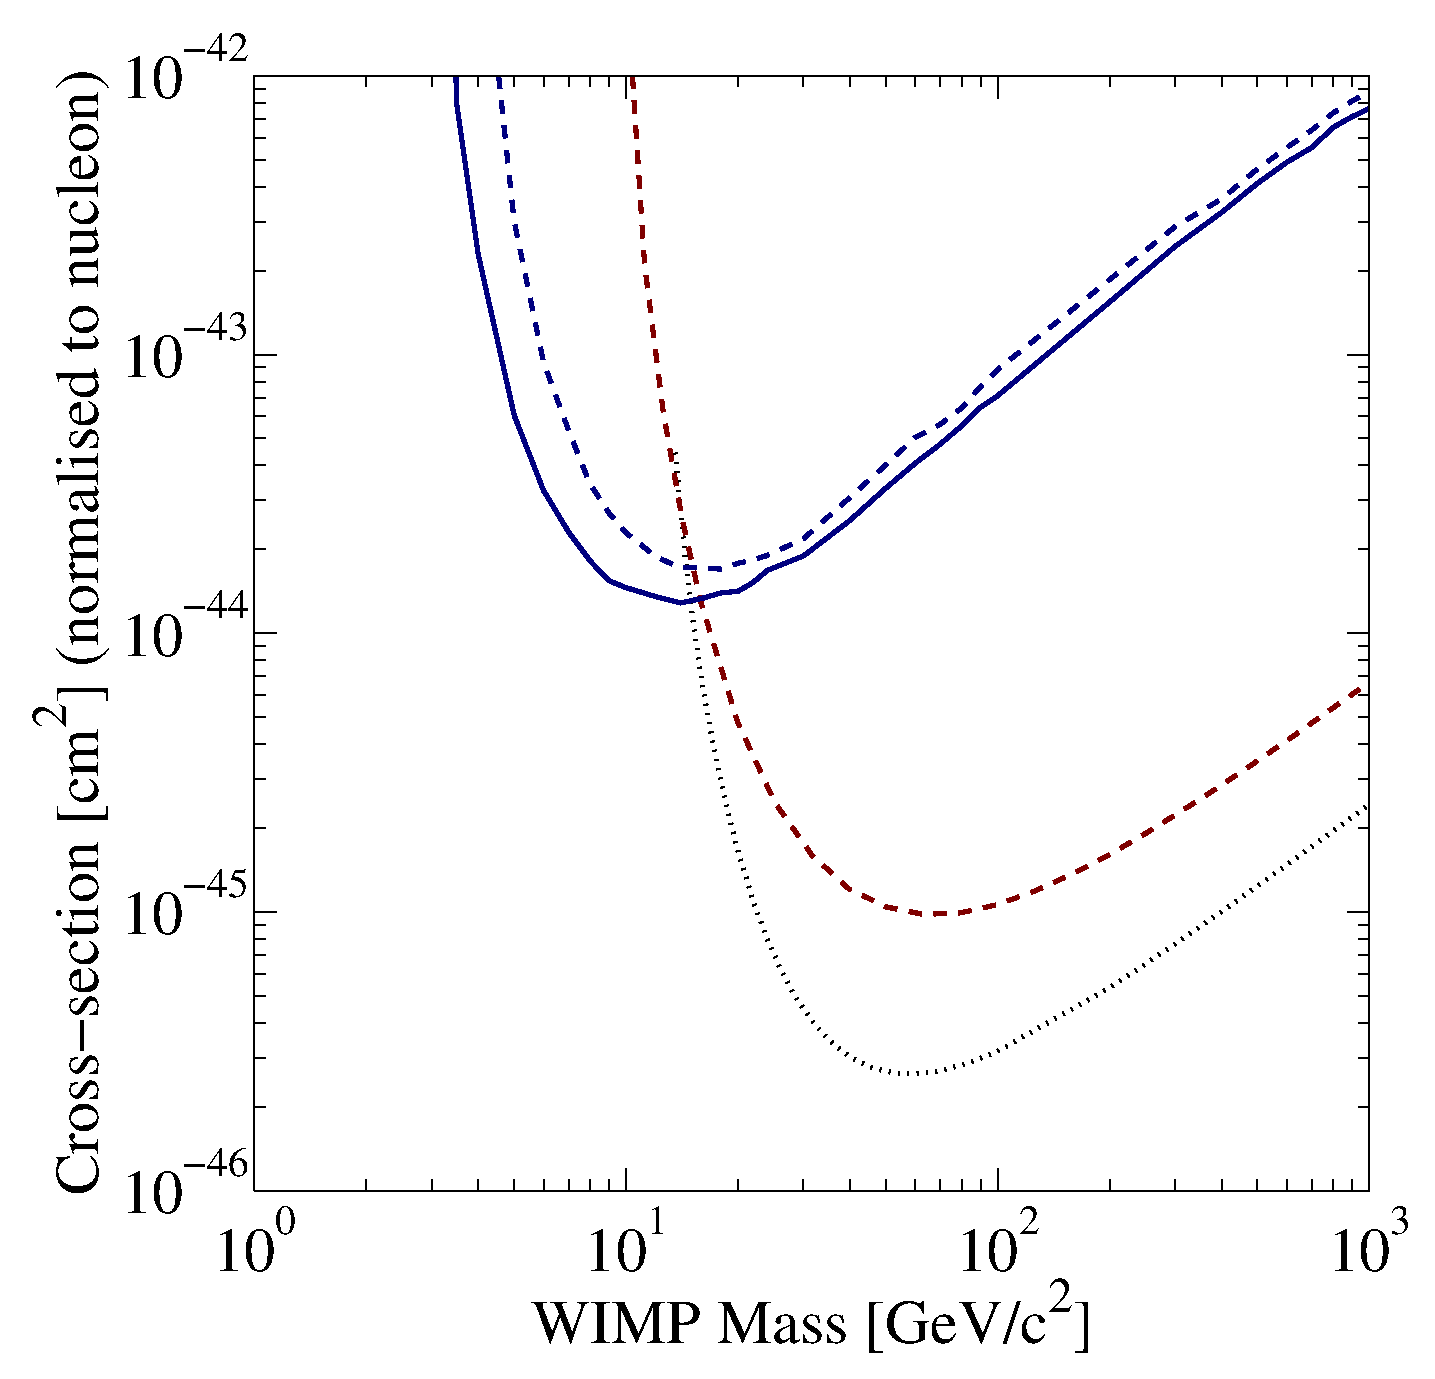
\includegraphics[width=0.9\textwidth]{MGM_MJ_Sensitivity_Compare}
				\caption[\MJ~\minmod~sensitivity to a WIMP signal, comparing to other experiments]
				{\MJ~\minmod~sensitivity to a WIMP signal, comparing to other experiments.}
				\label{fig:MJSensitivityToWIMPCompare}
			\end{figure}			
			
		\subsection{Sensitivity to axioelectric effect}
		\label{sec:MJSensitivityToAxions}
		
			\begin{figure}
				\centering
				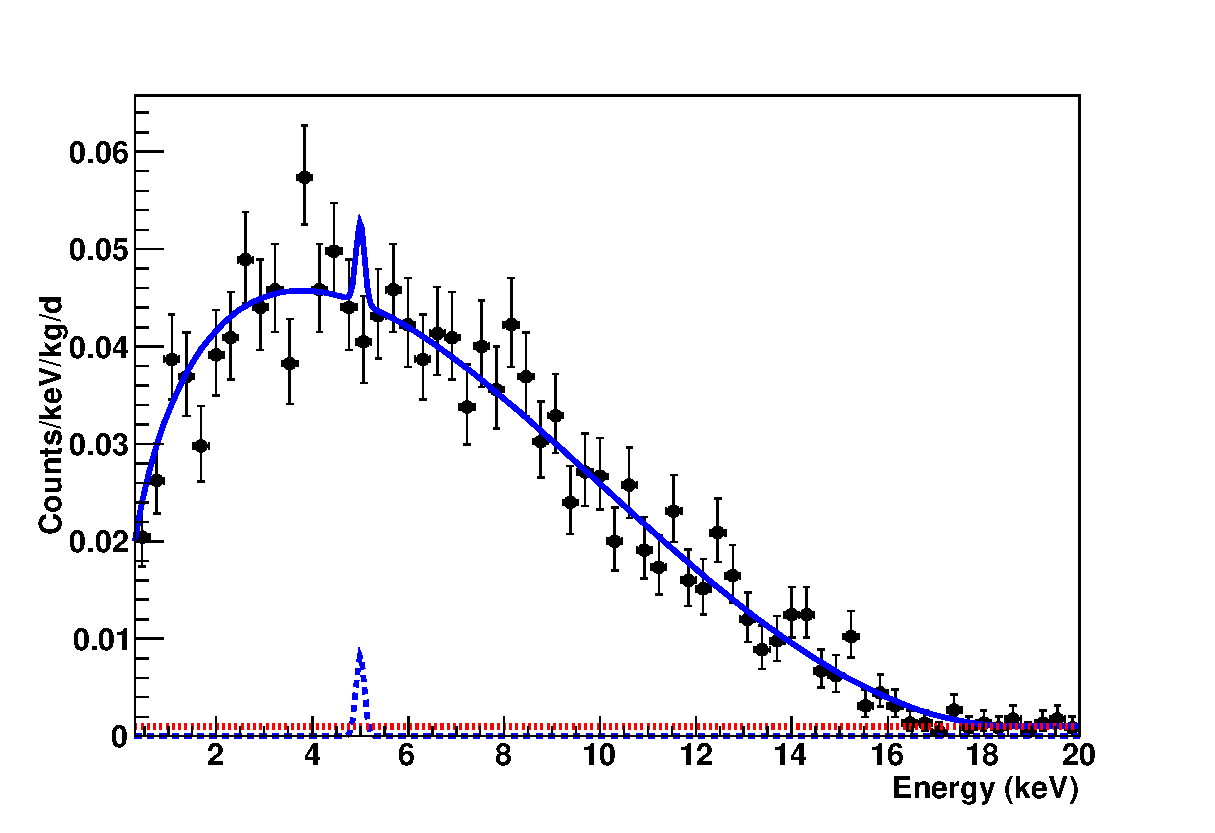
\includegraphics[width=0.9\textwidth]{MJDemoExampleSensFitAxion}
				\caption[\MJ~\minmod axioelectric sensitivity fit example.]{A sensitivity fit example 
				with axioelectric signal at $m_{a}=5$~keV, with $\gaa$ excluded at 90\% CL with
				value
				 $2.4\times10^{-11}$~pb.  Components of the fit are broken out including WIMP 
				 signal (blue dashed) and flat background (red dotted).  }
				\label{fig:MJSensitivityToAxionExample}
			\end{figure}
	
			\begin{figure}
				\centering
				\def\figheight{0.41\textheight}
				\subfigure[1~year (20 kg-yr) exposure time]{
					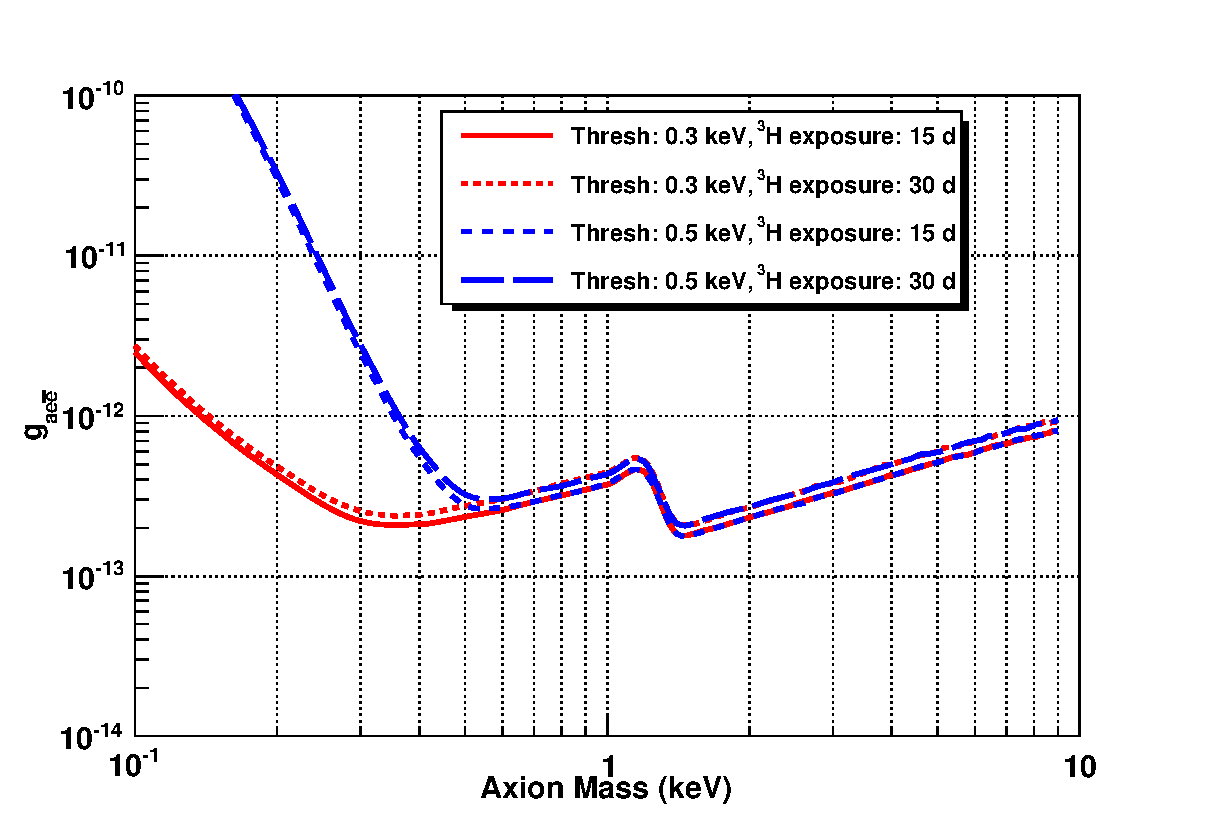
\includegraphics[height=\figheight]{1TimeExposureMJAxion}
					\label{fig:20TimeExposureMJAxion}						
				}
				\subfigure[5~year (100 kg-yr) exposure time]{
					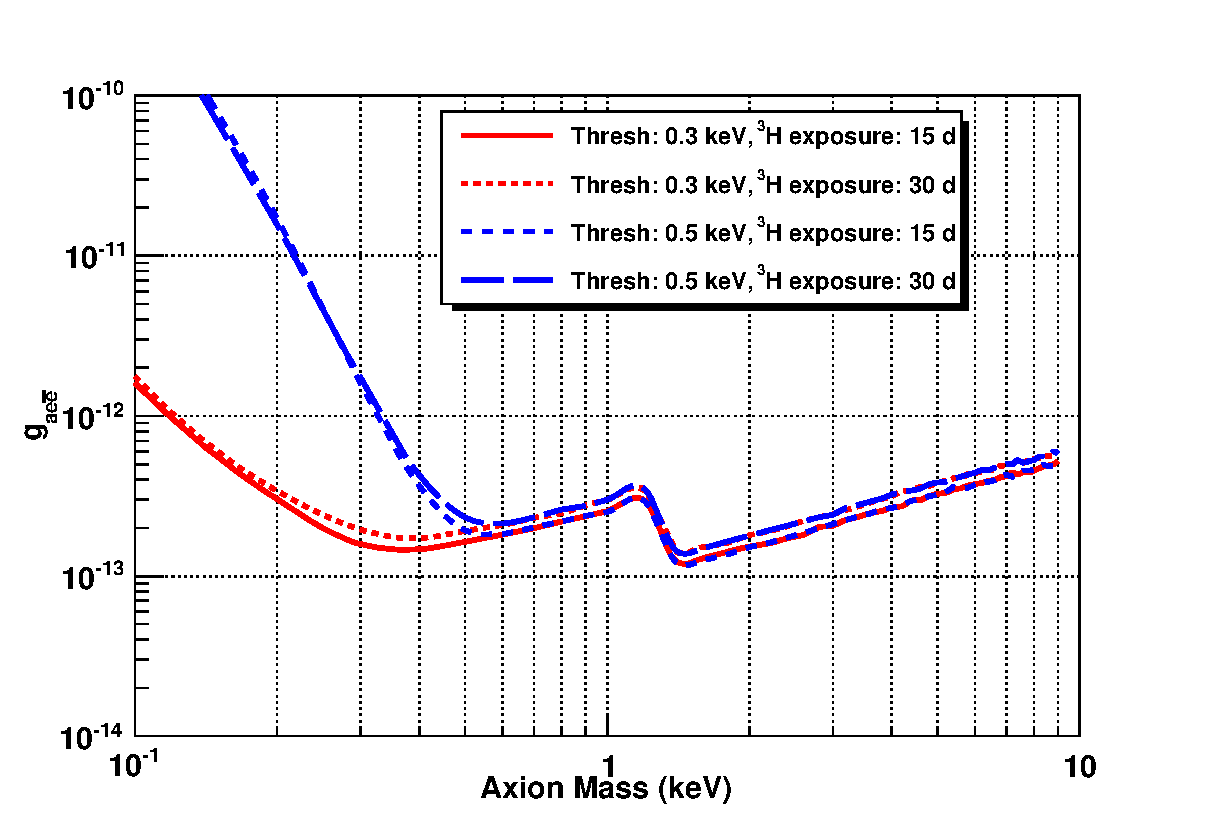
\includegraphics[height=\figheight]{5TimeExposureMJAxion}
					\label{fig:100TimeExposureMJAxion}						
				}				
				\caption[\MJ~\minmod~sensitivity to an axioelectric signal]{
				\MJ~\minmod~sensitivity to an axioelectric signal.}
				\label{fig:MJSensitivityToAxion}
			\end{figure}	
					
			\begin{figure}
				\centering
				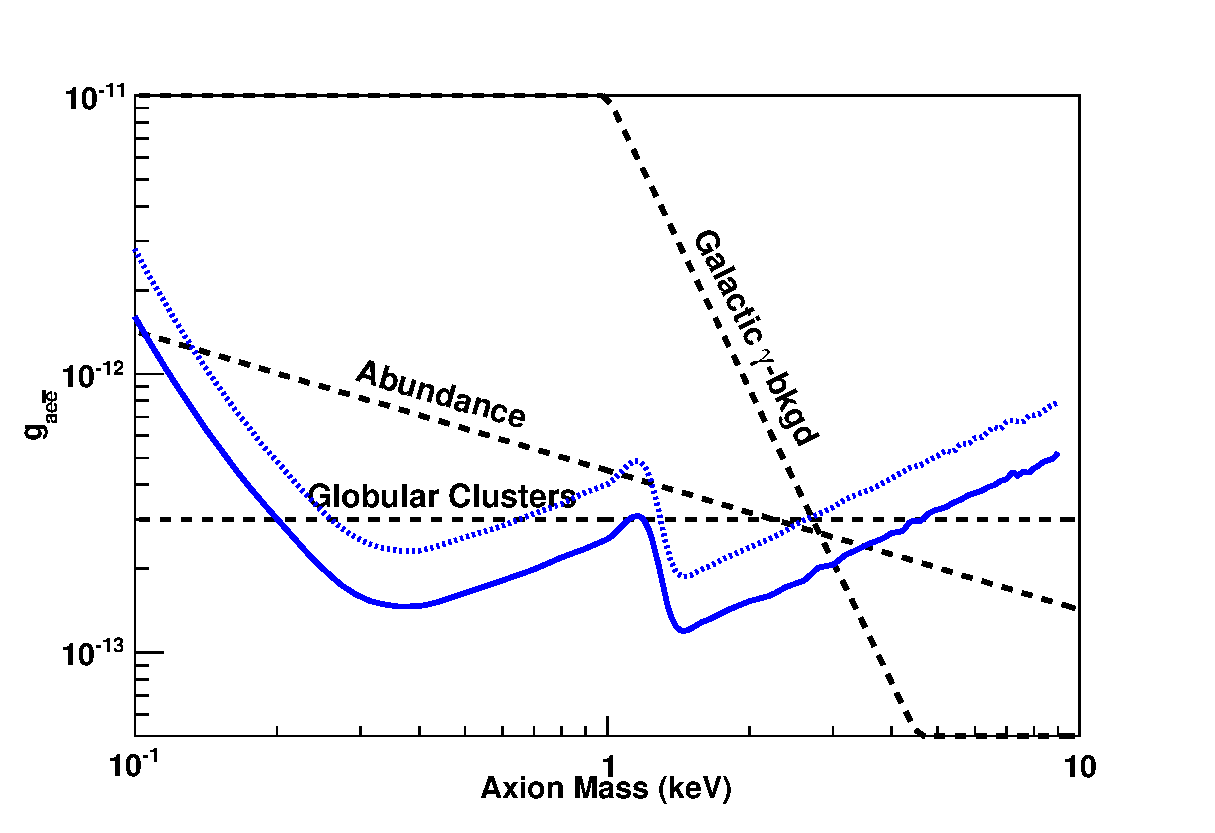
\includegraphics[width=0.9\textwidth]{MJAxionCompare}
				\caption{\MJ~\minmod~sensitivity to a Heavy Axion signal, comparing to other 
				experiments.}
				\label{fig:MJSensitivityToHeavyAxionsCompare}
			\end{figure}							

	\section{Conclusions}
	\label{sec:OtherLowEnergyConclusions}	